\section{Результаты работы}

Для проверки программы были рассмотрены обычные числа, отрицательное число,
случай округления, нуль, денормализованное число, бесконечность и
\texttt{NaN}. Результаты приведены в на рисунках с \ref{fig:default} по \ref{fig:corner_cases}

\subsection{Скриншоты запуска}

\begin{figure}[H]
    \centering
    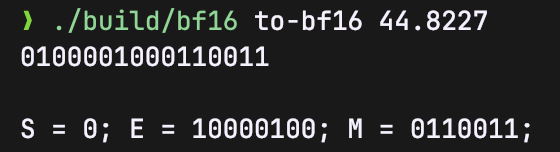
\includegraphics[width=0.5\linewidth]{myPhoto/default.png}
    \caption{Обычный случай \texttt{to-bf16}}
    \label{fig:default}
\end{figure}

\begin{figure}[H]
    \centering
    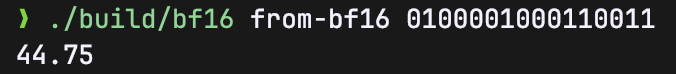
\includegraphics[width=0.5\linewidth]{myPhoto/default_to_bf16.png}
    \caption{Обычный случай \texttt{from-bf16}}
    \label{fig:default_to_bf16}
\end{figure}

\begin{figure}[H]
    \centering
    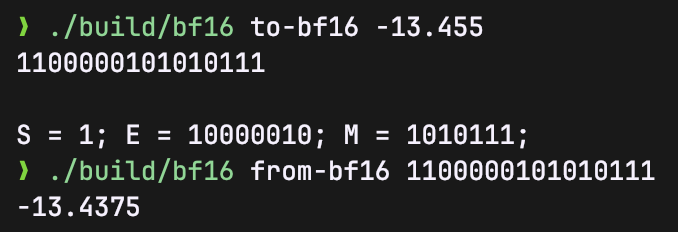
\includegraphics[width=0.5\linewidth]{myPhoto/with_minus.png}
    \caption{Значения с минусами}
    \label{fig:with_minus}
\end{figure}

\begin{figure}[H]
    \centering
    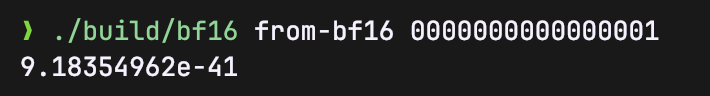
\includegraphics[width=0.5\linewidth]{myPhoto/minimal_int.png}
    \caption{Минимальное возможное число}
    \label{fig:minimal_int}
\end{figure}

\begin{figure}[H]
    \centering
    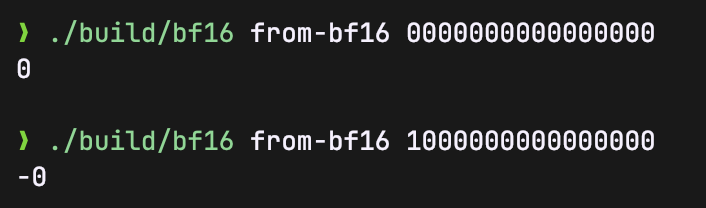
\includegraphics[width=0.5\linewidth]{myPhoto/null_with_sign.png}
    \caption{Нули со знаками}
    \label{fig:null_with_sign}
\end{figure}

\begin{figure}[H]
    \centering
    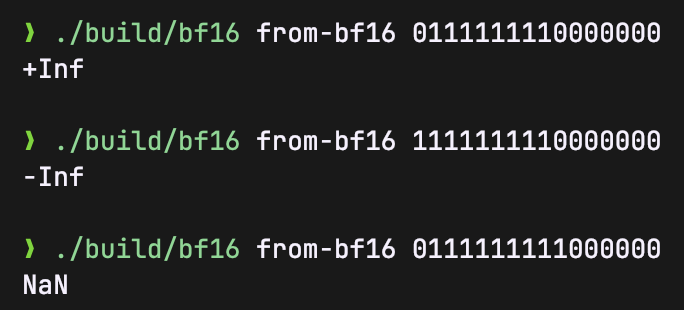
\includegraphics[width=0.5\linewidth]{myPhoto/corner_cases.png}
    \caption{Особые случаи}
    \label{fig:corner_cases}
\end{figure}
